\chapter{Memória}
De uma maneira geral, quando um processo é criado, sua imagem (ou parte dela) é armazenada em memória, onde a as instruções e os dados que estão sendo manipulados em um determinado instante são carregados na CPU. Os dados alterados são escritos em memória continuamente e os mais permanentes são armazenados em disco.

Um programa fonte apresenta instruções contendo endereços simbólicos, definidos pelo programador. Após o processo de compilação e montagem, o programa agora apresenta endereços relocáveis, construído em relação ao início do módulo onde são definidos. Após a \textit{linkagem}, o programa agora possui os endereços absolutos, único para o programa como um todo. Finalmente, com o \textit{loader}, quando o programa é carregado para a memória, os endereços físicos são efetivamente definidos. % TODO: ver se essa última sentença tá certa

















\section{Gerenciamento}
O gerenciamento de memória é implementado pelo \textbf{gerente de memória}, responsável por definir e implementar a política de gerenciamento de memória do SO. Além disso, independente desta política, o gerente deve controlar a alocação das porções de memória aos processos, liberando-as quando estas não forem mais necessárias. As técnicas de gerênciamento são três: \textit{monitor residente}, \textit{multiprogramação} e \textit{memória virtual}.






\subsection{Monitor Residente}
Em sistemas monoprogramados, a memória é geralmente dividida em duas áreas: uma para o usuário e outra para o sistema operacional.

Dessa forma, apenas um processo usuário está ativo por vez, pois a área de usuário é destinada a um processo apenas. Da mesma forma, a área do SO é ocupada por ele, o qual está sempre ativo.

Entretanto, é necessário um \textit{hardware} adicional, o qual vai impedir que processos de usuário invadão a área de memória do SO. É instaurada uma barreira, delimitando as áreas de memória, e a todo cálculo de endereço do processo usuário, o resultado é checado. A Figura \ref{fig:memory-fence} resume o processo.

\begin{figure}
  \centering
  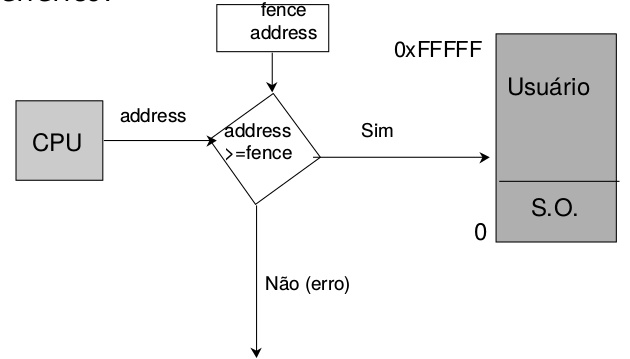
\includegraphics[width=0.65\textwidth]{memory-fence}
  \caption{O processo na CPU tentar acessar um endereço da memória. O \textit{hardware} checa se este endereço respeita o limite de área de memória do SO, liberando o acesso em caso positivo ou lançando um erro em caso negativo}
  \label{fig:memory-fence}
\end{figure}

Como \textbf{vantagens}, esta técnica tem implementação simples, pois só há um pequeno componente de proteção sendo usado. Além disso, os serviços do sistema operacional podem ser utilizados, como \textit{drivers}, interrupções, etc..

Como \textbf{desvantagem}, temos uma CPU sub-aproveitada, onde o sistema pode ser apenas mono-usuário e mono-tarefa






\subsection{Multiprogramação}
Multiprogramação é ofertada pela maioria dos computadores, onde vários processos coexistem na memória, havendo a necessidade da proteção de suas respectivas áreas de memória, evitando que um processo acesse a área de outro.

Logo, é lançado mão dos \textbf{registradores de base e limite}, definido dois limites de memória para o processo. Durante a execução, cada endereço usado para acessar a memória é adicionado ao valor contido no registrador de base, afim de obter o endereço físico onde o dado reside. Este registrador implementa a relocação.

Caso o endereço ultrapasse o valor do registrador limite, um erro é emitido. Assim, este registrador implementa a proteção de memória.







\subsection{Memória Virtual}
A memória virtual surgiu como uma solução para o problema de se alocar espaço em memória para um processo que não cabe inteiramente nela. Ou seja, temos um \textbf{processo com tamanho maior que o da memória física}.

A solução é quebrar o processo em unidades menores, carregando-as a medida que elas são necessárias. O problema é quem vai quebrar o processo: o programador ou o sistema operacional? Caso for o primeiro, temos um \textit{overlay} e do segundo, nasceu a memória virtual.

Proposto em 1961, é o método mais comum hoje em dia ao logo dos SO atuais, sendo um mecanismo genérico sendo suportado tanto por sistemas mono e multiprogramados. Logo, a idéia é referenciar mais endereços virtuais e não endereços físicos. Logo, parte do SO a responsabilidade de definir os módulos de memória e suas alocações.

\textbf{O número de endereços virtuais depende da capacidade de endereçamento da máquina} e do suporte do SO. Na execução de cada instrução, os endereços virtuais devem ser traduzidos para endereços físicos, o que exige um cálculo. Temos dois modelos para implementação da memória virtual:

\begin{itemize}
  \item \textbf{Paginação:} divide a memória física e a memória virtual em unidades de \textbf{tamanho fixo};

  \item \textbf{Segmentação:} divide a memória física e a memória virtual em unidades de \textbf{tamanho variável}.
\end{itemize}

Para ilustrar o possível espectro de endereços virtuais, supomos um arquitetura de 32 \textit{bits}. Logo, um processo pode endereçar até $2^{32} - 1$ endereços, independente da memória física.





\section{Espaço de Memória}

\subsection{Swapping}
\begin{definicao}{\textit{Swapping}}
  Movimento de processos \textbf{ativos} da memória para o disco e vice-e-versa.
\end{definicao}

Geralmente, a memória disponível no computador não é capaz de armazenar todos os processos ativos em um dado instante. Como não há espaço físico na memória, devemos colocar alguns processos ativos em disco. Normalmente, existe uma área em disco reservada para tal, chamada de \textbf{área de \textit{swap}}.

Definimos o movimento de memória para o disco como \textit{swap-out}. O movimento de disco para memória é o \textit{swap-in}.



\subsection{Alocação de Espaço}
O problema da alocação de espaço para processos é o problema de determinar a quantidade de memória que devemos reservar para um processo. Em sistemas onde um processo tem tamanho fixo, alocamos uma quantidade de memória exatamente igual ao tamanho do código binário do processo.

Infelizmente, a maioria dos sistemas permite que o tamanho da área de dados de um processo cresça ao longo da execução. Neste caso, é interessante alocar um espaço de memória maior que o tamanho inicial do processo, de forma a evitar o movimento do mesmo no caso de crescimento da sua área de dados.

Para tal, temos duas maneiras de implementar este controle: \textit{mapa de bits} e \textit{lista encadeada}.


\subsubsection{Mapa de \textit{Bits}}
Aqui a memória é dividida em unidade de alocação (\textit{UAs}) de tamanho fixo, onde cada uma corresponde a um \textit{bit} no mapa. Se a unidade estiver livre, o valor é 0, caso contrário, o valor é 1.

\begin{figure}[h]
  \centering
  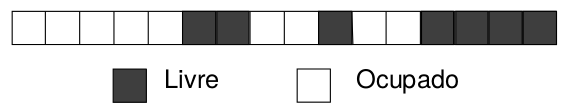
\includegraphics[width=0.5\textwidth]{memory-bitmap}
  \caption{Mapa de \textit{bits} associado à memória, com cadeia 1111100110110000}
  \label{fig:memory-bitmap}
\end{figure}


\subsubsection{Lista Encadeada}
Aqui as cadeias de segmentos livres e ocupados são representados através de um lista encadeada, onde cada entrada contém o tipo do segmento (livre ou ocupado), o endereço de início e um ponteiro para o próximo elemento. Desta forma, o percorrimento e busca por espaços é mais rápido.

Existem variações que implementam listas duplamente encadeadas, para que seja possível fazer o \textit{merge} de buracos. Tal situação é comum quando ocorre um término de processo.

\begin{figure}[h]
  \centering
  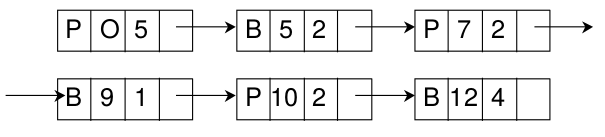
\includegraphics[width=0.6\textwidth]{memory-chained-list}
  \caption{Representação de lista encadeada para o contexto de memória da Figura \ref{fig:memory-bitmap}}
  \label{fig:memory-chained-list}
\end{figure}
















\section{Paginação}
Paginação é uma técnica de memória virtual, onde é utilizado um endereço virtual que representa um \textbf{espaço de endereçamento virtual} dividido em unidades de tamanho fixo, chamadas de \textbf{páginas}, e a memória física é dividida em unidades de tamanho fixo chamadas \textbf{\textit{page frames}}. Estas últimas, serão as áreas de memória física que irão abrigar as páginas utilizadas pela CPU.

A tradução entre páginas e \textit{frames} tem auxílio de um \textit{hardware} adicional, chamado \textbf{Memory Management Unit (MMU)}, o qual recebe um endereço virtual, mapeando-o no seu endereço físico correspondente, e escreve este último no barramento da memória, a qual poderá retornar o dado desejado para a CPU. A indexação de endereços é feita por uma estrutura interna da MMU chamada \textbf{tabela de páginas}.

\textbf{Nota:} se estas operações fossem feitas por \textit{software}, o esquema de paginação sera comprometido pelo alto \textit{overhead} a cada acesso.

\begin{figure}[h]
  \centering
  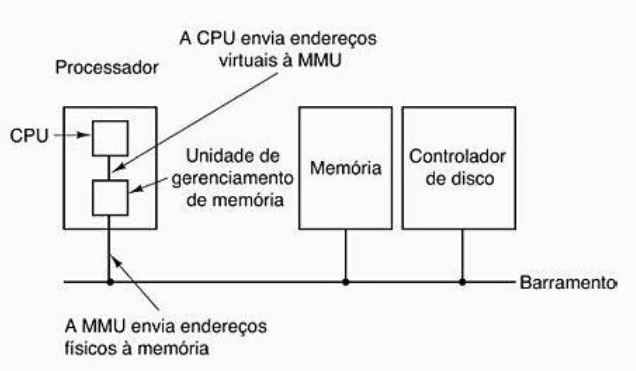
\includegraphics[width=0.75\textwidth]{pagination-overview}
  \caption{Esquema geral da paginação}
  \label{fig:pagination}
\end{figure}










\subsection{\textit{Page Fault}}
O espaço de endereçamento virtual é geralmente bem maior que o espaço de memória física. Dessa forma, é comum que uma página solicitada da CPU não esteja mapeada em memória física.

Por isso, a MMU possui em sua estrutura o \textit{bit} de presença, que indica a presença ou não da página na memória. Caso o \textit{bit} indique que não, a MMU irá \textbf{emitir um \textit{trap} para o SO, chamado de \textit{page fault}}.

Dessa forma, o SO irá escolher uma página da memória para ser substituída pela página requisitada. A página requisitada é buscada retirada do disco e inserida na memória, enquanto a página substituída é retirada da memória e inserida em disco. Por fim, a tabela de páginas é devidamente alterada, com a troca do \textit{bit} de presença e a instrução que gerou a requisição da memória é reexecutada. a Figura \ref{fig:page-fault} ilustra o processo.

\begin{figure}
  \centering
  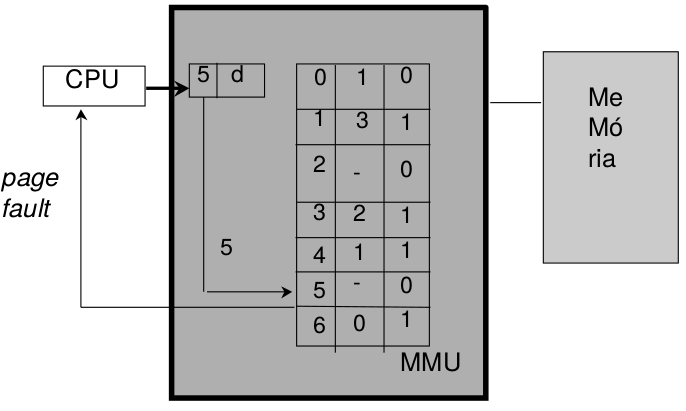
\includegraphics[width=0.7\textwidth]{page-fault}
  \caption{Esquema geral de um \textit{page fault}}
  \label{fig:page-fault}
\end{figure}











\subsection{Tabela de Páginas}
\begin{definicao}{Tabela de Páginas}
  Estrutura de dados presente na MMU que guarda as informações necessárias para o mapeamento do endereço virtual de um processo em endereços físicos.
\end{definicao}

As tabelas de página podem variar entre máquinas diferentes, porém possuem campos comuns:
\begin{itemize}
  \item \textbf{\textit{Bit} de \textit{cache}}: indica se a página pode ser colocada em \textit{cache};

  \item \textbf{\textit{Bit} de referência:} indica se a página foi referenciada;

  \item \textbf{\textit{Bit} de modificação:} indica se a página foi alterada;

  \item \textbf{\textit{Bit} de proteção:} indica a proteção associada à página;

  \item \textbf{\textit{Bit} de presença:} indica se a página está mapeada em memória física;

  \item \textbf{Número do \textit{frame}:} número do \textit{frame} onde a página está mapeada.
\end{itemize}

Observe que \textbf{o tamanho da tabela de páginas depende do espaço de endereçamento da arquitetura}. Dessa forma, a tabela poderia assumir espaços irreais como $2^64$. Dessa forma, dois problemas são inseridos: não é viável manter a tabela totalmente na MMU e a velocidade de mapeamento dos endereços pode ser comprometida.

Para mitigar o problema do tamanho, a \textbf{tabela de páginas fica armazenada em memória principal}, onde um registrador guarda o endereço de início desta tabela. Logo, a MMU utiliza uma memória associativa chamada de \textbf{\textit{Translation Look-aside Buffer} (TBL)}, onde algumas entradas da tabela de páginas são armazenadas.

Assim, quando um endereço virtual é apresentado a MMU, ela procura este na TBL. Se estiver presente, o mapeamento é direto, caso contrário, um acesso à memória é feito para recuperar a entrada da tabela de páginas. A entrada requisitada é inserida na TBL, de forma que futuras requisiçõe serão imediatas.

Temos duas organizações possíveis para a tabela de páginas: mapeamento direto ou invertida.

\subsubsection{Mapeamento Direto}
Também chamada de \textit{forward-mapped}, aqui a \textbf{tabela de páginas é um vetor de entradas armazenadas em memória}. Existe uma entrada para cada página e a \textit{frame} é obtida a partir desta.

Para este esquema \textbf{cada processo tem uma tabela de páginas}. Aliado ao crescimento do espaço de endereçamento e tamanho da página, as tabelas acabam por ficarem grandes demais. Dessa forma, para evitar que essas tabelas fiquem em memória o tempo todo, os computadores implementam as \textbf{tabelas de página em  multinível}.

Esta organização faz com que mesmo que um processo possa armazenar $2^n$ posições em memória física, ele não vai fazer isto. Logo, o número da página é quebrado em $n$ partes, onde $n$ será o número de níveis. A Figura \ref{fig:forward-mapped} ilustra a divisão.

\begin{figure}[h]
  \centering
  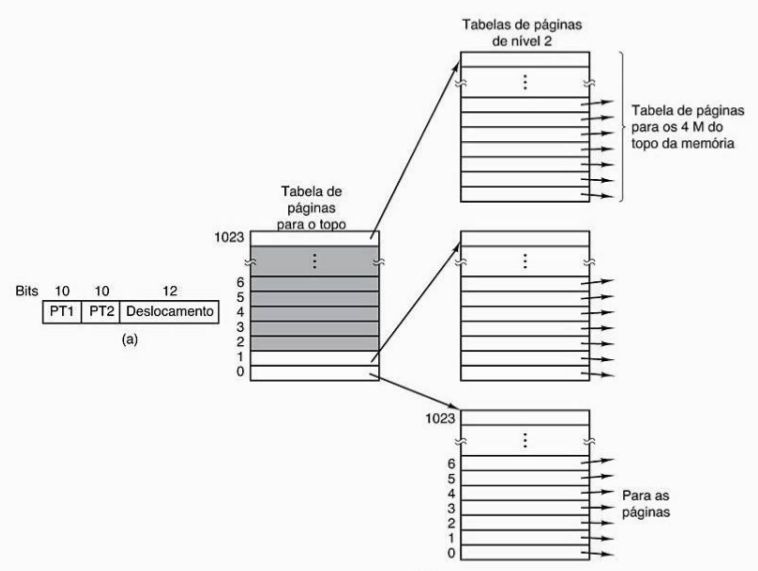
\includegraphics[width=0.8\textwidth]{forward-mapped}
  \caption{Tabelas de página de dois níveis, para um enderaçmento de 32 \textit{bits}}
  \label{fig:forward-mapped}
\end{figure}

Como exemplo, existem tabelas de páginas de 1 nível (PDP-11), 2 níveis (VAX), 3 níveis (SunSPARC) e 4 níveis (Motorola 68030). Além de 4 níveis, o projeto fica extremamente complexo e o ganho não é muito grande.




\subsubsection{Mapeamento Invertido}
Com processadores em 64 \textit{bits} e páginas com $4KB$, acabamos por ter $2^52$ entradas na tabela de página, o que torna inviável a utilização de tabelas com mapeamento direto. \textbf{Nota:} mesmo assim. algumas arquiteturas de 64 \textit{bits} utilizam este mapeamento, com 3 níveis.

Em tabelas de páginas invertidas, a indexação é feita pelo \textit{frame} e não mais pela página. O problema é que o índice utilizado pela CPU ainda é a página $p$. Por isso, neste método é utilizada uma tabela de \textit{hash}, com o \textit{frame} como índice. Logo, a CPU ainda envia $p$ como entrada, porém antes de ser aplicado na tabela, é feito um \textit{hash} sobre $p$ para obter o índice correspondente.

Entretanto, existem páginas que após o \textit{hash} acabam por cair no mesmo índice. Nelas, são criados \textit{buckets} com o endereço da página virtual $p$ e o \textit{frame} $f$ correspondente a ser escrito no barramento.
% TODO: rever isso com a Alba. Isso foi uma explicação do Tanenbaum (pg. X) e parece estar em desacordo com o slide












\subsection{Substituição de Páginas}
A condição de um bom algoritmo de substituição é de escolher sempre a página a página que está em memória física que será referenciada no futuro mais distante. Entretanto, isso não é possível pois não há como saber o futuro. Portanto, usamos estratégias realizáveis.

\subsubsection{NRU}
Abreviação de \textit{Não recentemente utilizada}, este método utiliza os \textit{bits} de referência ($R$) e de modificação ($M$). contidos na tabela de página.

O \textit{bit} $R$ sempre é setado para 1 quando a página associada for acessada, tanto para leitura como escrita. O \textit{bit} $M$ é setado para 1 sempre que a página for modificada, ou seja, apenas escrita. Todas estas atualizações são feitas em \textit{hardware}.

Quando o contexto do processo é carregado, os dois \textit{bits} são zerados e periodicamente, o SO zera o \textit{bit} R. Logo, quando há um \textit{page fault}, o SO analisa as páginas e as categoriza da seguinte forma:

\begin{itemize}
  \item \textbf{Classe 0:} não referenciada, não modificada ($R = 0 \mid M = 0$);

  \item \textbf{Classe 1:} não referenciada, modificada ($R = 0 \mid M = 1$);

  \item \textbf{Classe 2:} referenciada, não modificada ($R = 1 \mid M = 0$);

  \item \textbf{Classe 3:} referenciada, modificada ($R = 1 \mid M = 1$);
\end{itemize}

Dessa forma, o SO escolhe a página não-vazia da classe mais baixa e a substitui.

\textbf{Nota:} observe que para ter uma página não referenciada, mas modificada, é preciso que o SO tenha zerado o \textit{bit} de referência, o que ele faz periodicamente.



\subsubsection{FIFO}
Abreviação de \textit{first in, first out}, o FIFO usa a política de substituição da página que foi carregada a mais tempo. As páginas em memória são mantidas em uma fila organizada por idade. A página mais antiga no início e mais recente no final.

Quando ocorre o \textit{page fault}, a página removida é aquela que está no início da fila e a página que causou o \textit{page fault} é colocada no final.

Apesar de ser um algoritmo simples de se implementar, nada garante que uma página carregada a muito tempo não seja mais utilizada, dado que a utilização da página não está relacionada com o seu tempo de carga. Por isso, este algoritmo é raramente utilizado.




\subsubsection{Segunda Chance}
Este algoritmo é uma modificação do FIFO. Quando há um \textit{page fault}, o algoritmo analisa a página carregada há mais tempo. Se o seu \textit{bit} $R$ for 0, a página é escolhida para substituição. Entretanto, se $R$ for 1, o mesmo é zerado e a página colocada no final da fila, ou seja como mais recente. A busca continua até que haja uma página onde $R$ seja 0 e esta é escolhida.

Dessa forma, vemos que o algoritmo procura uma página que tenha sido carregada a muito tempo e não tenha sido referenciada. Se todas as páginas tiverem sido referenciadas, ele degenera para um FIFO.


\subsubsection{Relógio}
Utiliza a mesma filosofia do algoritmo de segunda chance, porém não utiliza filas simples para armazenar as páginas. As páginas são mantidas em uma fila circular, com um ponteiro que aponta para a página mais antiga.

Quando há um \textit{page fault}, o algoritmo analisa a página apontada pelo ponteiro. Se o seu \textit{bit} $R$ for 0, a página é escolhida para substituição. Caso seja 1, o \textit{bit} é zerado e o ponteiro aponta para a próxima página. A busca continua até que haja uma página onde R seja 0. A diferença está na substituição: a página inserida não é posta no fim de uma fila, mas assume a posição da página retirada.



\subsubsection{LRU}
Dado o princípio da localidade, páginas muito referenciadas nas últimas instruções tem grande chance de serem referenciadas pelas instruções futuras. Da mesma maneira, páginas não referenciadas há muito tempo tem grande probabilidade de continuarem a não serem utilizadas por muito tempo.

Portanto, o \textit{Least Recently Used} (LRU) se aproveita deste princípio e tenta escolher a página que foi referenciada no passado mais distante para ser substituída.

Teoricamente, ele tem bons resultados, mas sua implementação é custosa, dado que é necessário implementar uma lista encadeada organizada pelo tempo de último acesso. Dado isso, algumas técnicas de implementação do LRU acabam utilizando um \textit{hardware} especial. Entretanto, para SOs genéricos, o mais comum é a simulação de \textit{software} do LRU, que é chamada de \textit{Não Frequentemente Utilizada}, ou NFU.

No NFU necessitamos de um contador adicional, a ser mantido em tabela de páginas, para página. Periodicamente, o SO percorre todas as páginas em memória, adicionando o valor do \textit{bit} R de cada página ao seu contador. Quando ocorre um \textit{page fault}, página escolhida é aquela que possui o menor contador.

O problema do NFU é que uma página muito referenciada há muito tempo atrás raramente é escolhida para substituição, pois o NFU não "esquece" tais referencias passadas.


\subsubsection{NFU com \textit{Aging}}
Para que as referência antigas do NFU sejam esquecidas, devemos utilizar uma técnica chamada \textit{aging}. O número de \textit{bits} no contado é o número de referências passadas que será considerado.

No \textit{aging}, a cada interrupção de \textit{clock}, é feito um \textit{shift} do contador de cada página para a direita e o \textit{bit} R é inserido à esquerda, ou seja, no \textit{bit} mais significativo. Quando há um \textit{page fault}, o algoritmo escolhe a página com o menor contador. A Figura \ref{fig:nfu-aging} mostra o funcionamento.

\begin{figure}[h]
  \centering
  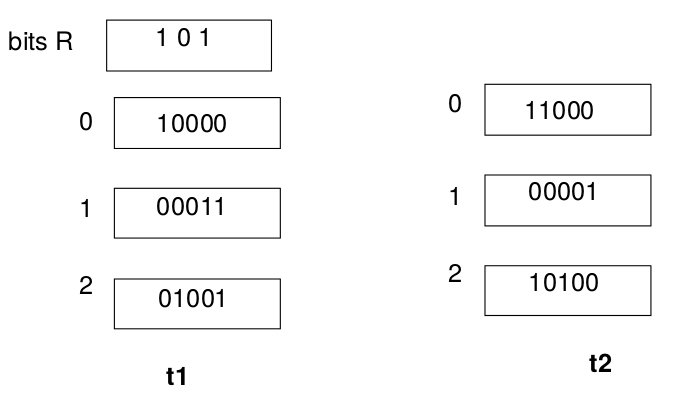
\includegraphics[width=0.7\textwidth]{nfu-aging}
  \caption{\textit{Shift} do NFU em dois tempos distintos adjacentes}
  \label{fig:nfu-aging}
\end{figure}




\subsection{Tratamento de \textit{Page Fault}}
Aqui é explicada toda a rotina de tratamento de um \textit{page fault}:

\begin{enumerate}
  \item O \textit{hardware} gera um \textit{trap} para o \textit{kernel} e salva o PC corrent na pilha;

  \item O \textit{hardware} executa uma rotina em código de máquina, que salva os demais registradores e outras informações. No final, a rotina chama o SO;

  \item O SO recebe o \textit{trap} e determina que ocorreu um \textit{page fault}. O mesmo determina a página virtual necessária para a resolução do \textit{page fault}, o qual geralmente está em um registrador especial;

  \item Com o endereço virtual em falta, o SO verifica se o endereço é válida e se houve a violação de proteção;

  \item O SO determina um espaço de \textit{frame} livre para inserir a página solicitada. Caso não haja, o algoritmo de subtituição é executado. Se a página selecionada tiver sido modificada, ela deve ser escrita em disco. O \textit{frame} é marcado como reservado e o SO escolhe um novo processo para rodar;

  \item Quando o SO tem certeza de que o \textit{frame} está livre, ele determina o endereço de disco onde se encontra a página que causou o \textit{page fault}. Durante a busca no disco para a passagem para a memória, um novo processo é posto para rodar;

  \item Ao checar a interrupção de disco que indica o términa da cópia da página de disco para memória, a tabela de páginas é alterada e o \textit{frame} é marcado como ocupado;

  \item A instrução que causou o \textit{page fault} é carregada no registrador de instruções e o seu endereço é carregado no PC. Daí, o processo desta instrução é colocado para rodar. O SO termina a execução, voltando a ser executada a rotina em código de máquina que o chamou. A rotina restaura os registradores e demais informações para a situação anterior à falta e dá o processador ao processo de usuário;

\end{enumerate}








\subsection{Funcionamento Detalhado}
Aqui descrevemos o funcionamento geral do pedido de uma página pela CPU. Supondo um processo na CPU que requisite um dado da memória:

\begin{enumerate}
  \item A CPU envia o endereço virtual $v$ à MMU;

  \item Na MMU, o endereço virtual é divido em uma tupla ($p,d$), onde $p$ é a página desejada e $d$ o deslocamento dentro da página;

  \item Ainda na MMU, a página $p$ é utilizada para acessar a \textbf{tabela de páginas}, que reside na MMU. A partir dessa tabela, a tupla inicial é convertida na tupla $F = (F,d)$ correspondente do endereço físico. Nela, $f$ corresponderá ao \textit{frame} da memória física e o deslocamento permanece o mesmo;

  \item Antes de escrever o endereço no barramento, a MMU checa se a página está mapeada em memória física, através de um \textit{bit} de presença.

  \begin{itemize}
    \item Caso a página esteja mapeada, o endereço já pode ser escrito no barramento;

    \item Caso contrário, a MMU gerá um \textit{syscall} ao SO, chamado de \textbf{\textit{page fault}}. Dessa forma, seleciona um \textit{frame} da memória pra ser substituído pela página requisitada e a instrução inicial de acesso a memória é reexecutada. Consequentemente, a MMU vai constatar que a página existe;
  \end{itemize}

  \item O endereço físico $F$ é escrito no barramento de memória
\end{enumerate}


\subsubsection{Cálculos na Paginação}
Em uma arquitetura com espaço de endereçamento de $b$ \textit{bits}, páginas de tamanho $P$ \textit{bytes} e uma memória RAM com tamanho $M$ \textit{bytes}, temos que:

\begin{itemize}
  \item O número de endereços virtuais possíveis é de $2^b$;

  \item O número $F$, que é o total de \textit{frames} na RAM é dado por:

  \begin{equation*}
    F = \frac{M}{P}
  \end{equation*}
\end{itemize}

Ao solicitar um endereço virtual à memória, a CPU utiliza a tupla $(p,d)$, onde $p$ é a página virtual e $d$ o deslocamento dentro da página. Este endereço virtual deve ser transformado em um endereço físico \textbf{de mesmo tamanho}, composto pela tupla $(f,d)$, onde $f$ é o número do \textit{frame} a ser utilizado e $d$ é o mesmo deslocamento usado no endereço virtual.

Disso, temos que:

\begin{itemize}
  \item O tamanho de página $P$ é o valor máximo que $d$ pode assumir;

  \item
\end{itemize}
